% !TeX encoding = UTF-8
% !TeX root = V7_Lichtbeugung.tex
% !TeX spellcheck = de_DE_frami



%\textsf{He-Ne}-Laser mit Wellenlänge $\lambda=633$\,nm
%Linse $L_1$ mit Brennweite $f_1=199\pm2$\,mm
%Linse $L_2$ mit Brennweite $f_1=151\pm2$\,mm
%CCD-Kamera mit Pixeln der Größe $9\,\micro\metre \times 9\,\micro\metre$


% \usepackage[free-standing-units]{siunitx}
% \sisetup{locale = DE}					% fuer deutsche Dezimaltrenner und Aufzaehlungen
% \DeclareSIUnit\px{px}

\section{Auswertung}

\subsection{Versuchsaufbau und Versuchsziele}

\begin{figure}[h]
\centering
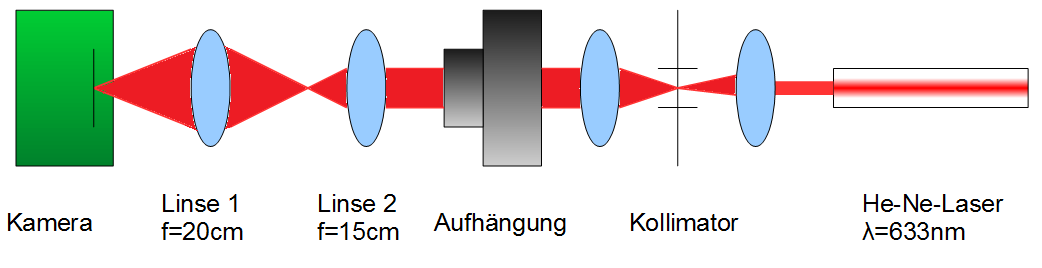
\includegraphics[width=\textwidth]{versuchaufbau.png}
\caption[Versuchsaufbau]{Schematische Darstellung des Versuchsaufbaus. Der Strahl eines Helium-Neon-Lasers (\textsf{He-Ne}-Laser) wird mit Hilfe eines Kollimators zu einer Punktquelle begrenzt, aufgeweitet und parallelisiert. Hierzu besteht der Kollimator aus zwei bikonvexen Linsen und einer Lochblende, welche zwischen den Linsen positioniert ist. Die erzeugten parallelen Strahlen durchlaufen eine Aufhängung, in welche verschiedene Objekte eingesetzt werden können. Für die Beugungsmuster im Fourierraum wird nur Linse 1 mit Brennweite $f_1=20\,\centi\metre$ benutzt, dessen Fourierebene direkt auf dem Detektionsmedium liegt. Für eine echte Abbildung wird Linse 2 mit $f_2=15\,\centi\metre$ zwischen Linse 1 und Aufhängung platziert.}
\label{aufbau}
\end{figure}

Der Versuchsaufbau, welcher für den Versuch Lichtbeugung benötigt wird, ist schematisch in Abbildung \ref{aufbau} illustriert. Die benötigte photonische Einstrahlung basiert auf einem Helium-Neon-Laser mit einer Wellenlänge $\lambda=633\,\nano\metre$. Im Strahlengang wird ein Kollimator positioniert, um aus einem kontinuierlichen Laserstrahl eine Punktquelle zu erzeugen. Mit Hilfe der zweiten Kollimator-Linse wird ein paralleler Strahlengang hergestellt. Weiter werden bis auf die erste Beugungsordnung der Blende alle höheren Ordnungen durch die Aufhängung ausgeblendet. Für die Bildgebung (genauer: echte und Fourier Abbildung) wird nun diese zentrale Ordnung durch das Objekt geleitet. Die montierten Bilder, außer Einstein- und Bikini Model-Bild, können schematisch in der nächsten Abbildung \ref{Masken} gesehen werden.

\begin{figure}[h]
\centering
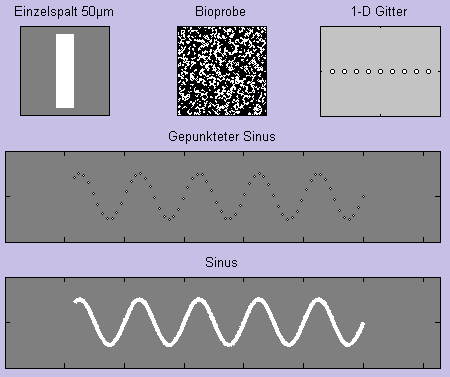
\includegraphics[width=0.95\textwidth]{Masken.png}
\caption[Maskenformen]{Schematische Darstellung der montierten Bildmasken}
\label{Masken}
\end{figure}

Im Rahmen des Experiments sind drei Messung durchgeführt worden. Dabei wurden die Brennweiten der Linsen (1) und (2) überprüft. Weiter wurde die Spaltbreite eines Einzelspaltes bestimmt und zuletzt Beugungsbilder sowie Abbildungen der Masken in Abbildung \ref{Masken} aufgenommen.

Zu Beginn des Experiments wurde eine komplette Neu-Justierung des Systems vorgenommen, da bei einer schlechten Justage u.a. die Brennweitenbestimmung der Linsen (1) und (2) durch optische Fehlerquellen ungenau wird. Die erhaltenen Brennweiten sind in der nachfolgende Tabellen (\ref{Brennweite}) eingetragen.

\begin{table}[hb]
	\centering
	\caption[]{Resultate der Brennweiten Bestimmung}
	\begin{tabular}{ccc}
		\toprule
				& Brennweite $f$ in mm 	& 	Fehler in mm	\\
		\midrule
		Linse 1	& 199				&	$\pm1$		\\
		Linse 2	& 151				&	$\pm2$		\\
		\bottomrule
	\end{tabular}
	\label{Brennweite}
\end{table}

Die Messresultate sind überraschend gut und bedürfen keiner weiteren Diskussion.
% Allerdings ist zu erwähnen, dass bei früher Messungen die Brennweiten nicht mit der Herstellerangabe übereinstimmten. Es wurde herausgefunden, dass dieser Effekt durch schlechte Justierung hervorgerufen wird. Dieses Problem genügt einer simplen Erklärung. Bei schlechter justage wird sphärische Abberation und dadurch eine Brennweiten Verfälschung erzeugt, bezogen auf Brennweite Messungen mit monochromatischen und paraxialen Wellen.

\section{Spaltbreitenbestimmung} \label{Spaltbreitenbestimmung}
Die zweite Aufgabe im Experiment ist die Spaltbreiten Bestimmung eines Einzelspaltes. Zu diesem Zweck dient die Intensitätsverteilung des Einzelspalt Beugungsbilds in Abbildung \ref{ESpaltBeugung} und Formel \eqref{eq:Messung}.
\begin{figure}[h]
\centering
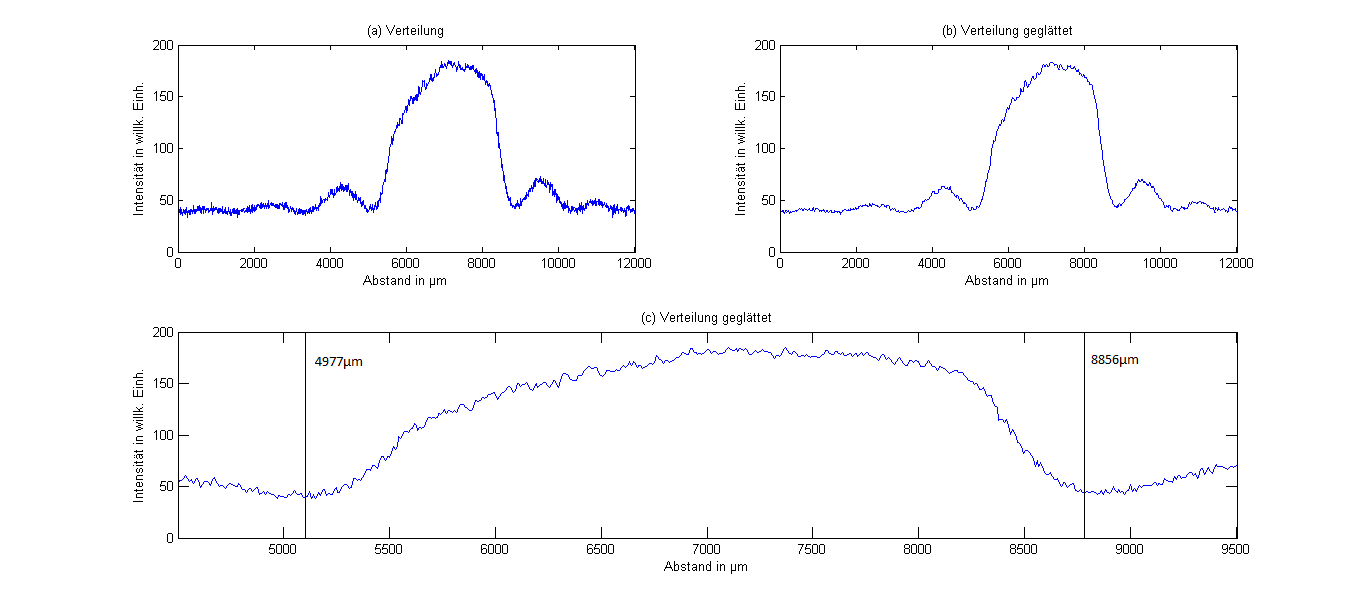
\includegraphics[width=\textwidth]{verteilung.png}
\caption[Intensitätsverteilung]{Intensitätsverteilung bei Beugung an einem Einzelspalt. Es zeigt, wie erwartet, den Verlauf eines Sinus Cardinalis. Die Position null µm gibt einen Rand des Chips an. Abbildung (a) illustriert die unbearbeiteten Daten. In Abbildung (b) wurde die Kurve geglättet. Abbildung (c) ist eine Vergrößerung von (b) um die erste Beugungsordnung.}
\label{ESpaltBeugung}
\end{figure}

Bekannten Messparameter sind die Wellenlänge $\lambda=633~\mathrm{nm}$ und der Abstand vom Spalt zum Schirm $s=35~cm\pm~\mathrm{1mm}$. Mit Hilfe der Intenistätsverteilung aus \ref{ESpaltBeugung} ergibt sich die Breite des ersten Maximum mit $b=3,879~\mathrm{mm}\pm 0,05~\mathrm{mm}$. Mit Hilfe der Gleichung \eqref{eq:Messung} ergibt sich eine Spaltbreite von $d=60~\mathrm{\mu m}\pm80~\mathrm{\mu m}$. Der errechnete Wert beträgt nicht gerundet $57\mathrm{\mu m}$ und liegt in der Nähe der Angabe des Herstellers von $50~\mathrm{\mu m}$. Problematisch ist der berechnete Fehler. Dieser Umstand hat einen simplen Grund. Die beiden ersten Minimas um den ersten Maximum wurden improvisorisch mit Hilfe eines Matlab Skriptes bestimmt. Das Problem bei diesem Verfahren ist das Rauschen im Signal. Dabei kann es vorkommen, dass ein versetztes Minimum gefunden wird. Deshalb wurde hier der Fehler auf $50~\mathrm{\mu m}$ geschätzt und der berechnete Fehlerwert kann vernachlässigt werden.

\section{Fourier-Beugungen und echte Abbildungen}
Die letzte Aufgabe war die Erstellung von Beugungsbildern sowie echte Abbildungen der in Abbildung \ref{Masken} gezeigten Masken. Im folgenden werden die einzelnen Bilder vorgeführt und relativ kurz darüber diskutiert. Dabei wird die Reihenfolge echte Abbildung und Beugungsbild bei jeder einzelner Maske eingehalten.
\paragraph{Einzelspalt} Das durch die Vorlesung bekannte Muster eines Einzelspaltes wurde auch hier beobachtet. Dabei ist die Stellung des Spaltes in der Maske vertikal. Die horizontale Anordnung der Intensitätsverteilung im Beugungsbild (Fourierraum) entspricht der Theorie. Beide gemessene Bilder ergänzen sich zu einander. Dabei wurde in der echten Abbildung das Hintergrundrauschen nicht abgezogen, da diese die qualitativen Analyse nicht behindert. Im Beugungsbild wurde allerdings eine art exponentielle Krümmung beobachtet. Qualitativ kann dieser Fehler durch eine spährische Abberration und/oder ein schiefer Einfall in die Optik erklärt werden, da im Experiment eine nicht paraxialer Strahl benutzt wurde. Ebenso erkennt man eine auf der rechten Seite im Beugungsbild eine Aufspaltung des Maximas in zwei Linien. Diese Erscheinung ist nicht trivial. Der erste Erklärungsversuch wäre diese Linien als ein Resultat eines Diodenlaser zu sehen, da solche Laser einen ähnlichen Verlauf zeigen. Allerdings wurde im Experiment eine Gasentladungslaser benutzt. Eine weitere Erklärung wären, dass durch die eingestellte Optik zwei verschiedene Niveaus abgebildet wurden, wobei diese Aufgabe nicht trivial ist. Falls dies hier eingetreten ist kann dies nur aus purem Zufall eingetreten sein.

\paragraph{Bio-Probe} Weiter wurde eine Probe mit unbekannter Struktur und Materie untersucht, die hier Bio-Probe getauft wurde. Die echte Abbildung zeigt eine Vergrößerung an einem Punkt der Maske. Es sind vereinzelte Strukturen zu erkennen. Allerdings ist hier nicht klar, ob die Struktur in der Maske oder auf der Öberfläche sich befindet. Es kann nicht ausgeschlossen werden, dass die gemessenen Strukturen einfache Schmutzansammlungen auf der Oberfläche sind. Das Beugungsbild ist ebenso unbefriedigend. In Fourierraum wurden neben dem gezeigten Hauptmaximum, in Richtung diagonal rechts/oben ein weiteres INterferenzmaximum mit dem bloßen Auge beobachtet. Allerdings ist der direkte Abstand zu groß um beide in der Kamera zu erfassen. Daher wird nur das Hauptmaximum gezeigt. Ersichtlich ist eine konstruktive Interferenz nur am Laserspot.

\paragraph{1-D Gitter} Ein weiteres bekanntes Bild ist das ein Eindimensionale Gitter. Dabei entspricht die echte Abbildung dem Beugungsbild. Durch horizontale Anordnung der Punkte zu einem Gitter, werden alle horizontalen Interferenzen zu einander aufgehoben. Dabei überleben nur die vertikalen Interferenzen. Es ist theoretisch möglich die Lochgröße mit dem Beugungsbild zu bestimmen. Dies würde auf analogerweise, wie eine Spaltbreitenbestimmung eines Einzelspaltes geschehen. Es wurde allerdings im Rahmen des Experimentes nicht durchgeführt.

\paragraph{gepunkteter Sinus} Eine gepunktete Sinuskurve diente als Maske. Dabei ist das Beugungsbild sehr Interessant und erzeugt eine völlig unterschiedliche Struktur verglichen mit einem durchgehenden Sinus, welcher weiter im nächsten Paragraphen diskutiert wird. Das Beugungsbild zeigt im Zentrum mehrere zu einander verschobene kantige Sinusverläufe. Weiter außerhalb sind zwei in ihrer Intensität relativ schwache Beugungsringe zu beobachten. Verglichen mit einzelnen Messungen - jetzt im Gedankengang eine einzelne kleine Blende - sind diese Interferenzringe ein Effekt der einzelnen Punkte (oder auch im entfernten Sinne "Blende"). Das Zentrum des Beugungsbildes ist eine intensive Überlagerung der Sinusstruktur und vieler einzelner Punkte/Blenden. Mathematisch lässt sich bei einem Sinusverlauf die Differenz zweier Dirac-Distributionen, in der Form

\begin{equation}
	\mathcal{FT}(sin(x))=\frac{1}{i}(\delta(x-\omega_0)-\delta(x+\omega_0))~\mathrm{,}
\end{equation}
berechnen. Dies findet man im Beugungsbild. Man nehme sich einen hellen Punkt im Beugungsbild und laufen in horizontaler/vertikaler Richtung bis zu nächsten hellen Punkt. Diese beiden Punkte entsprechen dem positiven Beitrag der Dirac-Distribution. Die schwarze Punkt in der Mitte ist der negative Beitrag zur ersten Distribution. Theoretisch ist es möglich die Verschiebung $\omega_0$ durch die Distanz zwischen erster hellen und erster dunkel Distribution zu berechnen. Dabei ist eine Intensitätsverteilung, wie in \ref{Spaltbreitenbestimmung}. Allerdings wurde dies im Rahmen des Experiments nicht bestimmt.

\paragraph{Sinus} Zum weiteren Vergleich dient eine kontinuierliche Sinusform. Die Ergebnisse der Sinus Maske ist eine Vergrößerte Abbildung der Maske und das dazugehörige Beugungsbild. Aus der echten Abbildung ist eine nicht kontinuierlicher Sinus, sowie an einer Stelle eine Deformation im Verlauf ersichtlich. Für weitere Analysen wird an dieser Stelle ein kontinuierlicher Sinus angenommen. Das Beugungsbild gibt eine sehr schöne experimentelle Ergänzung zur Fourier Transformierten des Sinus. Dabei sind zwei gekreuzte Geraden zu erkennen. Jede dieser einzelnen Geraden kann zu einem Ergebnis eines Einzelspaltversuches aufgeteilt werden. Dabei erkennt man pro Gerade einen periodischen Wechsel zwischen Maxima und Minima. Dabei ist das Zentrum des Beugungsbildes eine Intensitätsüberlagerung beider Geraden. Des Weiteren ist hier genauso die mathematische Beschreibung des Fourier Transformierten Sinus wiederzufinden. Der imaginäre Faktor $i$ tritt durch die Winkeldrehung in Erscheinung.

\paragraph{Bikini-Model} Der Masken Favorit war die Bikini-Model Maske. Dabei wurde eine nicht schöne Abbildung erstellt, dafür ein besseres Beugungsbild. In der echten Abbildung musste etwas getrickst werden um eine relativ deutliche Abbildung zu messen. Die Abbildung erfolgte mit einer Distanz Verkürzung zwischen Kamera und der Linse (1), da bei theoretisch geforderten Positionierung nicht genug Intensität erhalten wurde. Ersichtlich ist die zu abbildende Bikini-Model und schiefe Streifen, welche Herstellungsbedingt sein sollten. Im Beugungsbild sind neben dem Hauptmaximum im Zentrum weitere gitterförmig angeordnet Punkte zu erkennen. Dabei ist nicht ganz klar, ob diese wirklich von den schiefen Streifen in der echten Abbildung kommen. Verglichen mit einem zwei Zweidimensionalen Beugungsgitter müssten die Struktur im Beugungsbild um einen bestimmten Winkel gedreht sein, da die Streifen in der echten Abbildung ebenfalls einen Winkel zu einer Achse aufzeigen. Daher ist es nicht auszuschließen, dass diese Winkelverschiebung bei einer Überlagerung mit einer relativ hübschen Frau in Bikini diese Winkeldrehung verschwindet. Interessant wäre eine Messung mit dem gleichen Bild mit dem Unterschied, dass diese Streifen in einem anderen Winkel auftreten. Weiter sieht man im Beugungsbild einen Abbildungsfehler. Die Beugungsordnungnen am rechten Rand weisen Koma artige Erscheinungen auf.

\paragraph{Einstein} Die letzte verwendete Maske ist das bekannte Einstein Beugungsporträt. Es wurde eine vergrößerte Version der Abbildung erstellt, wobei man Konturen und Gesichtszüge relativ gut erkennen kann. Das Beugungsbild entspricht der bekannten Form. Die Überlagerung von Gitterinformation und Bildinformation ist sehr gut zu erkennen. Dabei entsprechen alle intensiven Ordnungen Bildinformationen. Die zusätzlich auftretende Linienförmige Intensitätsverteilung entspricht einer horizontalen Gitterstruktur in der Maske. Weiter ist am Rande ein Abbildungsfehler der Art Koma zu erkennen. Weiter kann mit einer weiteren Blende zwischen Linse (1) und (2) die Dunkelfeldmethode bzw. Hellfeldmethode durchgeführt werden. Dabei würde bei ersteren die Konturen im Bild viel besser zu Geltung kommen. Die experimentelle Realisierung würde durch die weitere Blende stattfinden. Phänomenologisch würde man alle Ordnungen ausblenden bis auf hier einer der vier zweiten Beugungsordnungen. Analog die Hellfeldmethode besitzt sehr viel Intensität im Bild. Diese Methode betont weniger die Konturen im Bild. Erzeugt wird dieses Phänomen ebenfalls mit einer Blende, wobei nur das erste Hauptmaximum nicht ausgeblendet wird. Die Blende ist ebenfalls zwischen der Fourier- und der Abbildungslinse.


\newpage
\begin{figure}[h]
	\centering
	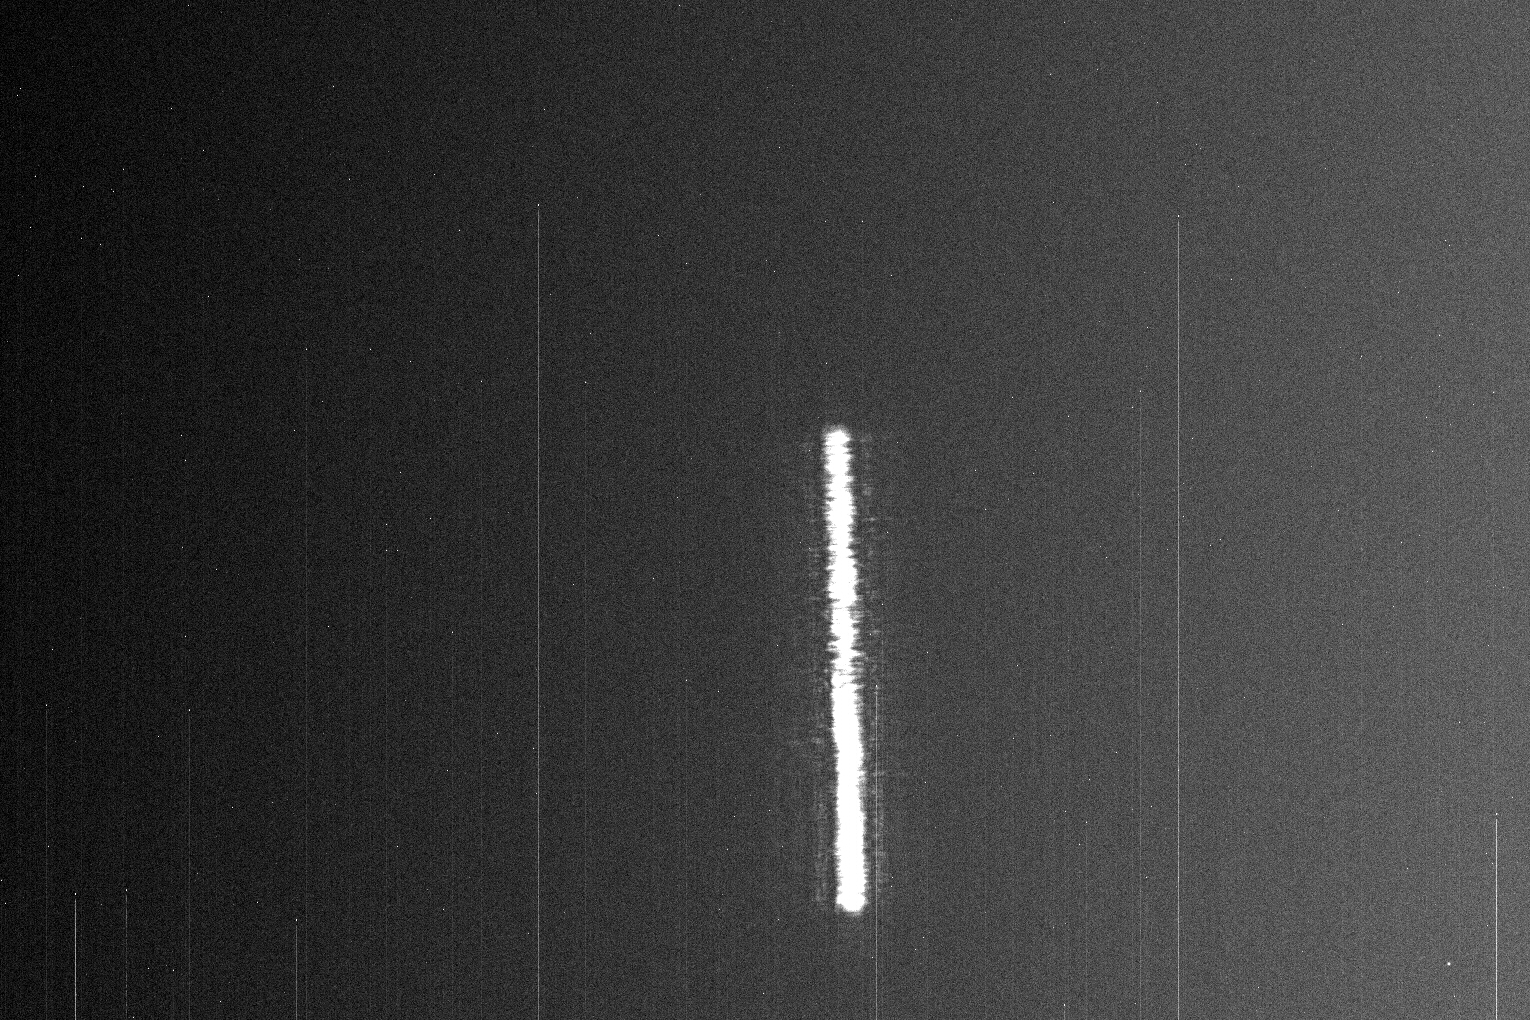
\includegraphics[width=\textwidth]{Daten/spalt_1.jpg}
	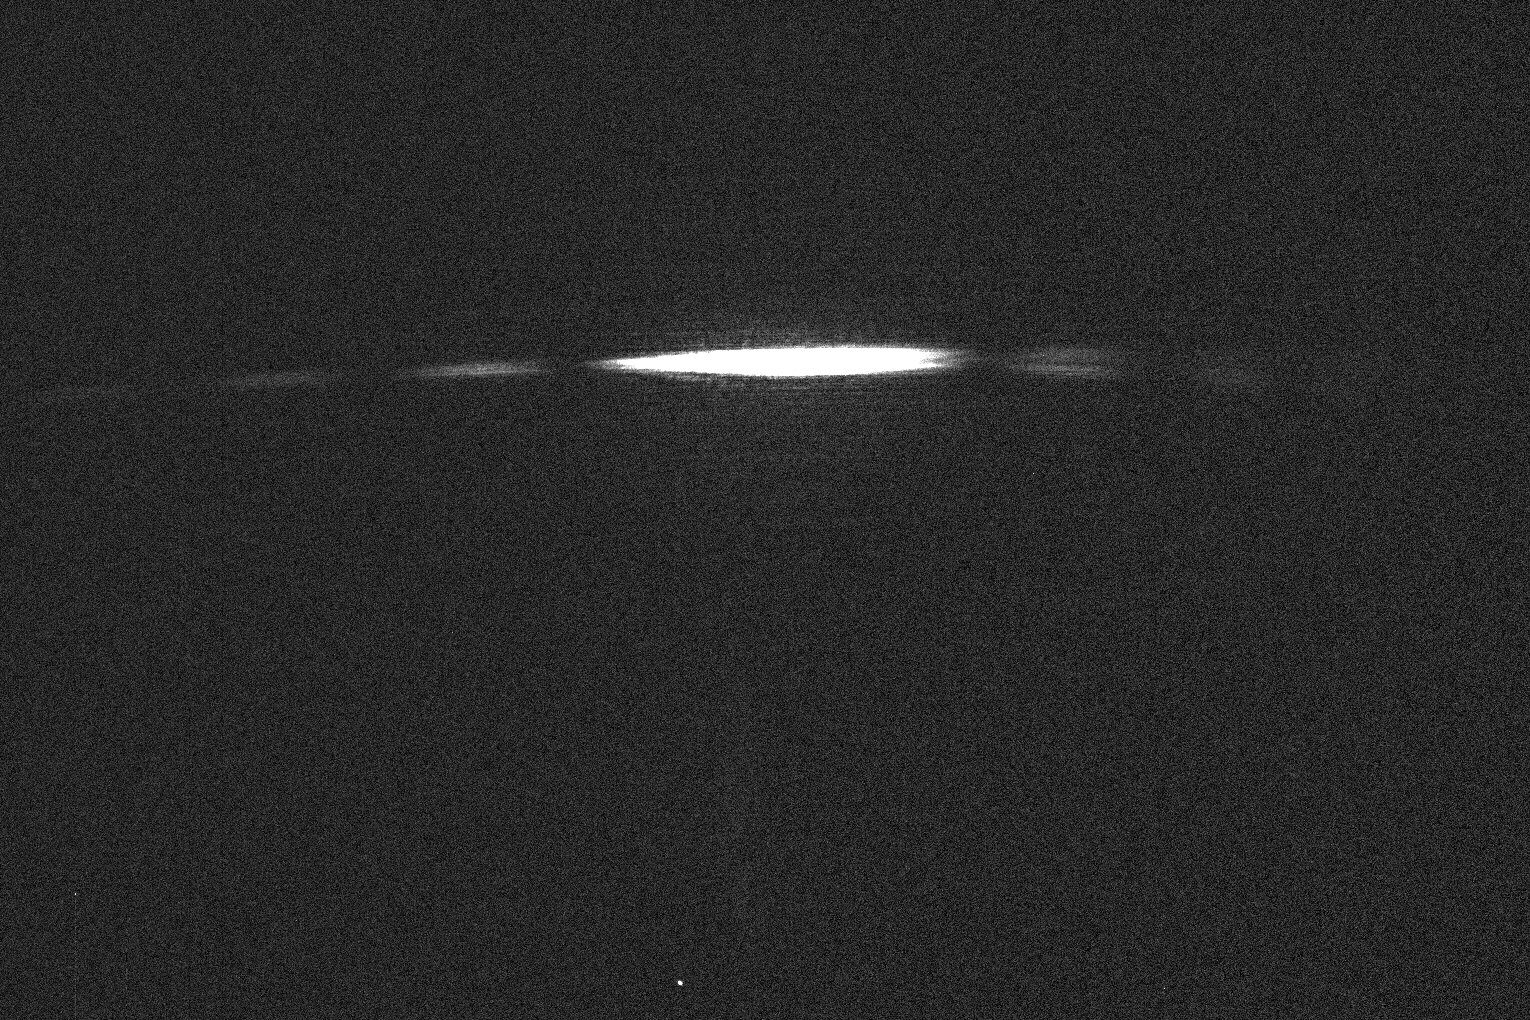
\includegraphics[width=\textwidth]{Daten/spalt_2.jpg}
	\caption[Aufnahme Einzelspalt]{Oben echte Abbildung Einzelspalt. Unten Beugungsbild}
\end{figure}

\begin{figure}[h]
	\centering
	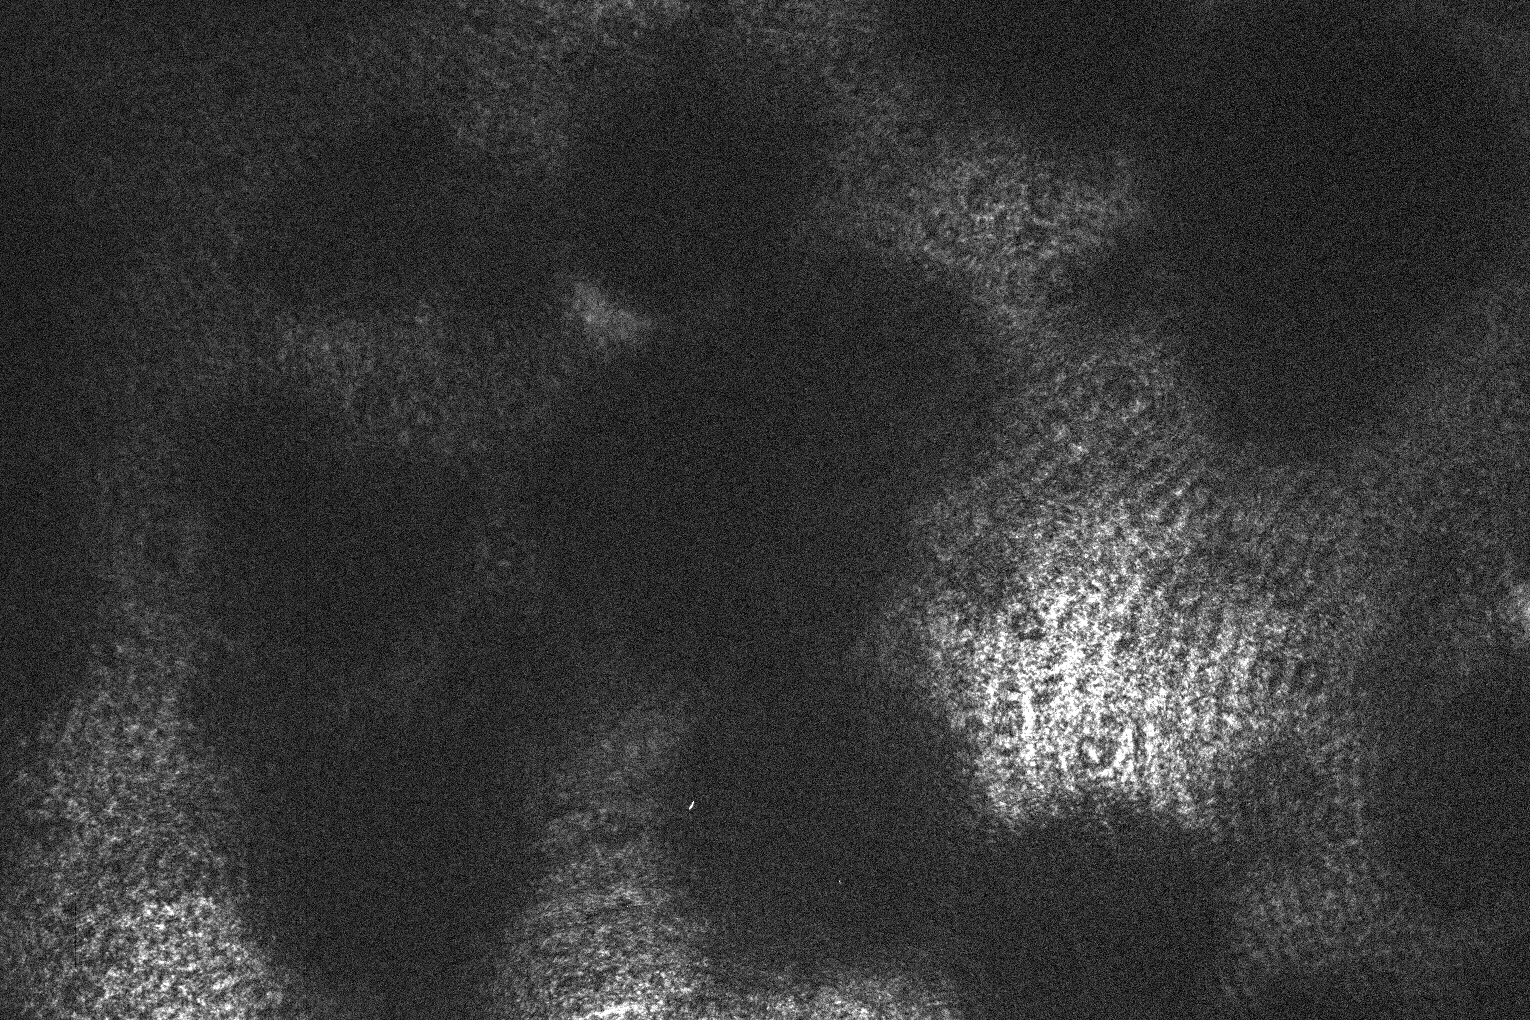
\includegraphics[width=\textwidth]{Daten/bio_1.jpg}
	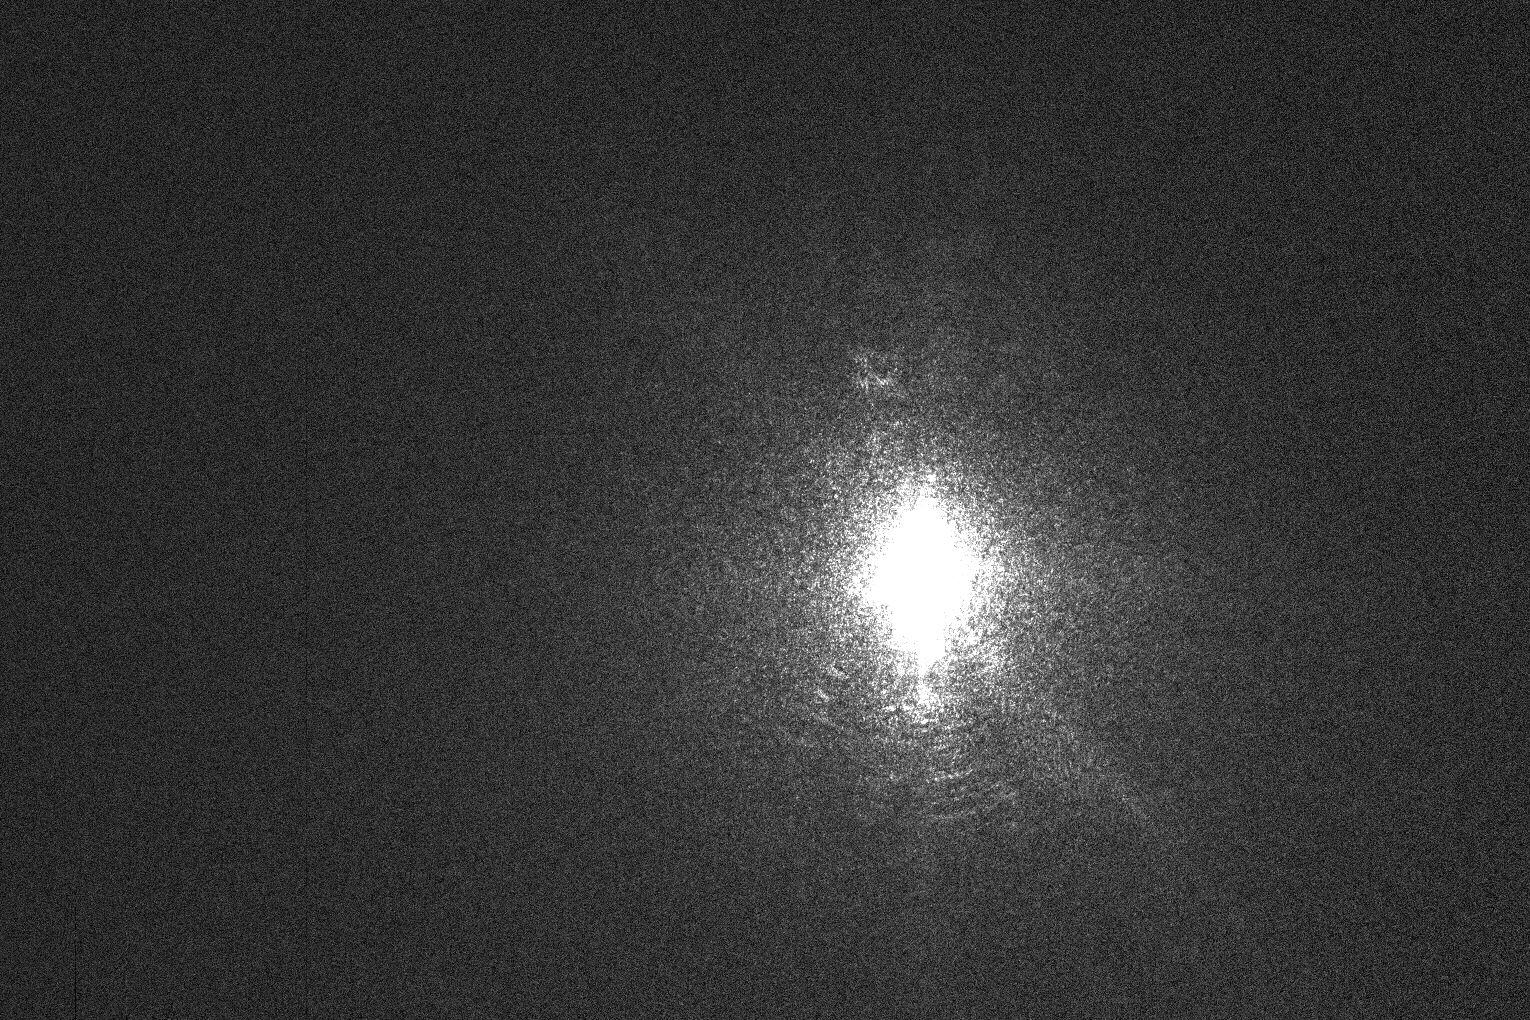
\includegraphics[width=\textwidth]{Daten/bio_2.jpg}
	\caption[Aufnahme biologische Probe]{Oben echte Abbildung unbekannten Probe. Unten Beugungsbild}
\end{figure}
\begin{figure}[h]
	\centering
	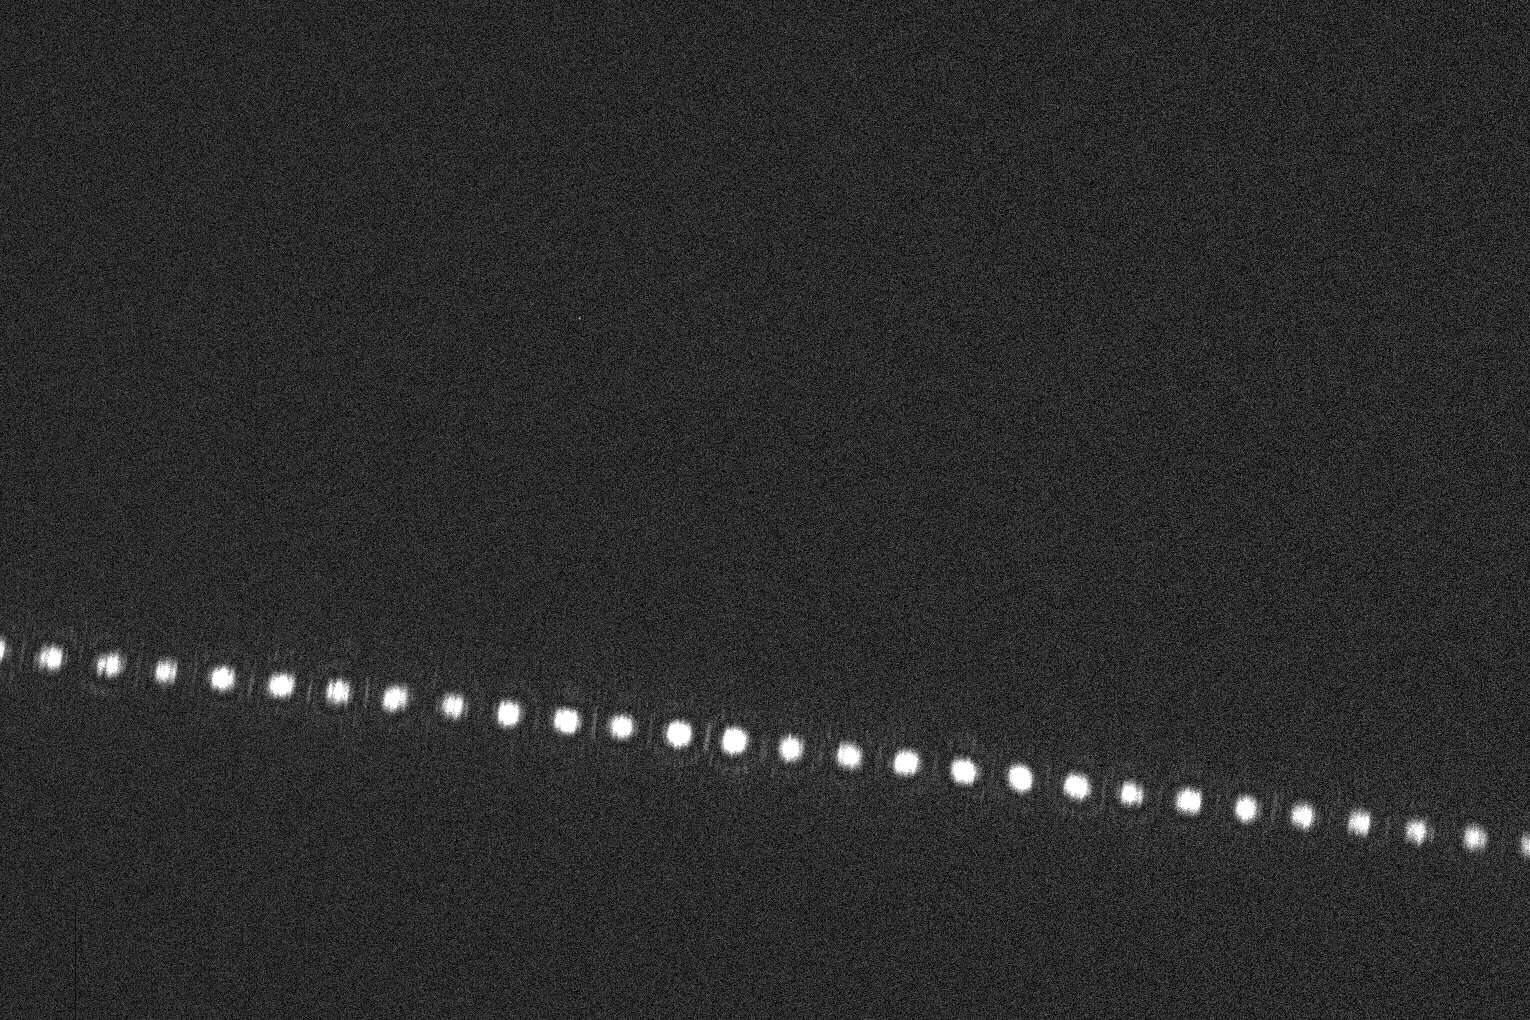
\includegraphics[width=\textwidth]{Daten/gitter_1.jpg}
	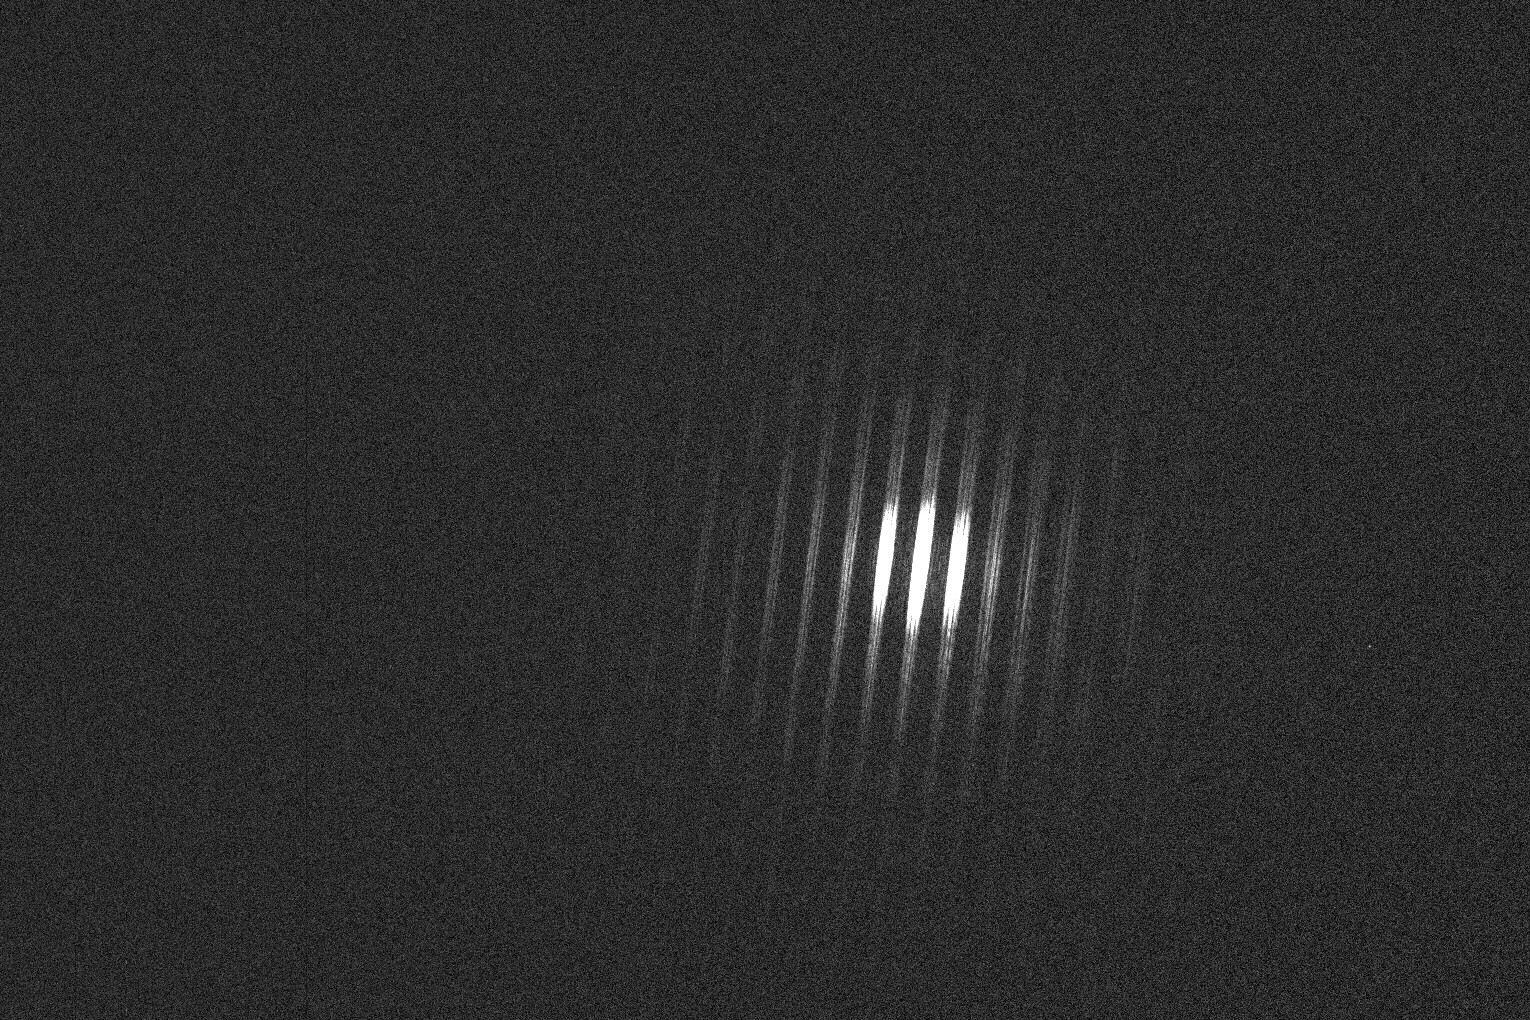
\includegraphics[width=\textwidth]{Daten/gitter_2.jpg}
	\caption[Aufnahme Punktgitter]{Oben echte Abbildung 1-D Gitter. Unten Beugungsbild}
\end{figure}

\begin{figure}[h]
	\centering
	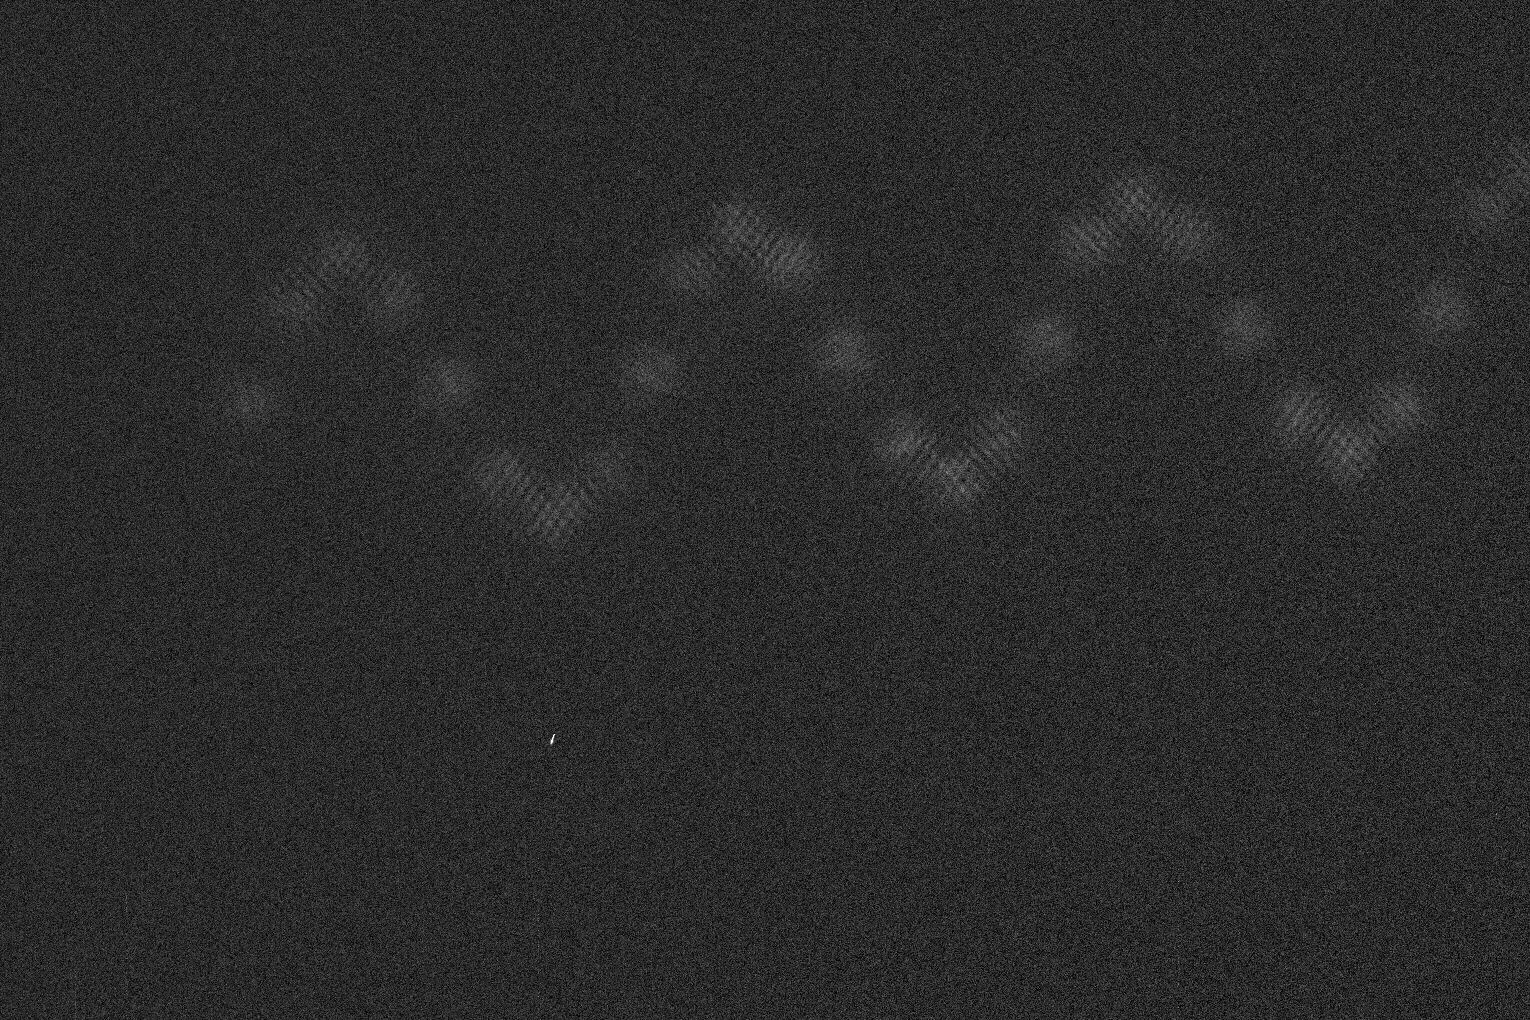
\includegraphics[width=\textwidth]{Daten/sindot_1.jpg}
	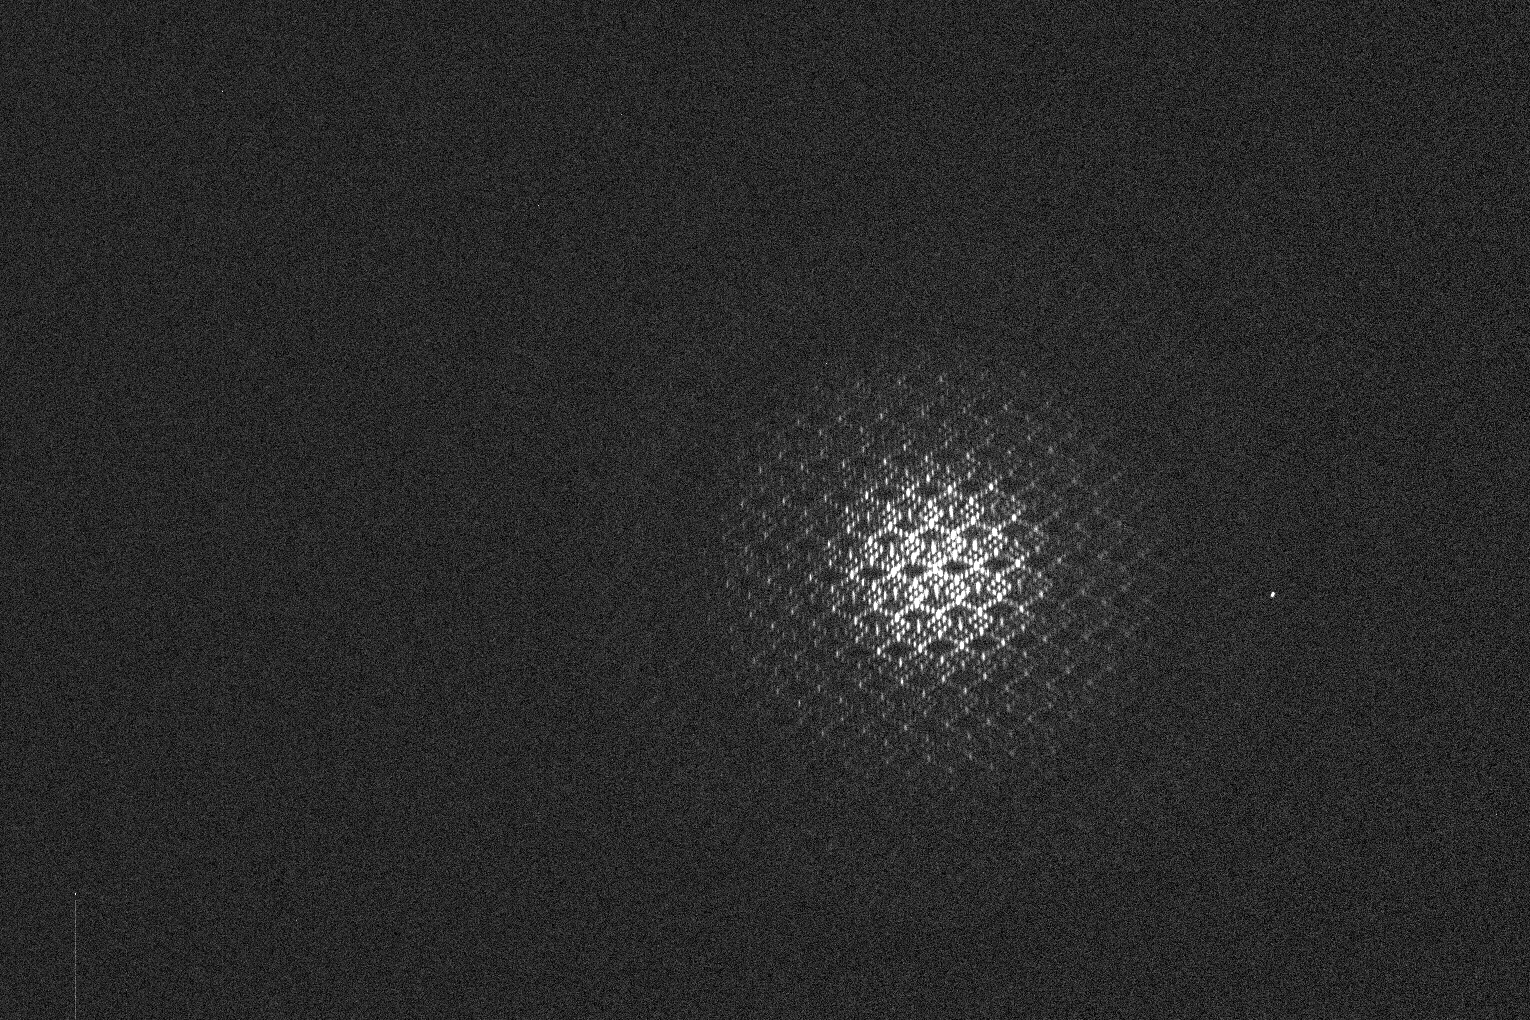
\includegraphics[width=\textwidth]{Daten/sindot_2.jpg}
	\caption[Aufnahme gepunkteter Sinus]{Ob
		en echte Abbildung gepunkteter Sinus. Unten Beugungsbild}
\end{figure}
\begin{figure}[h]
	\centering
	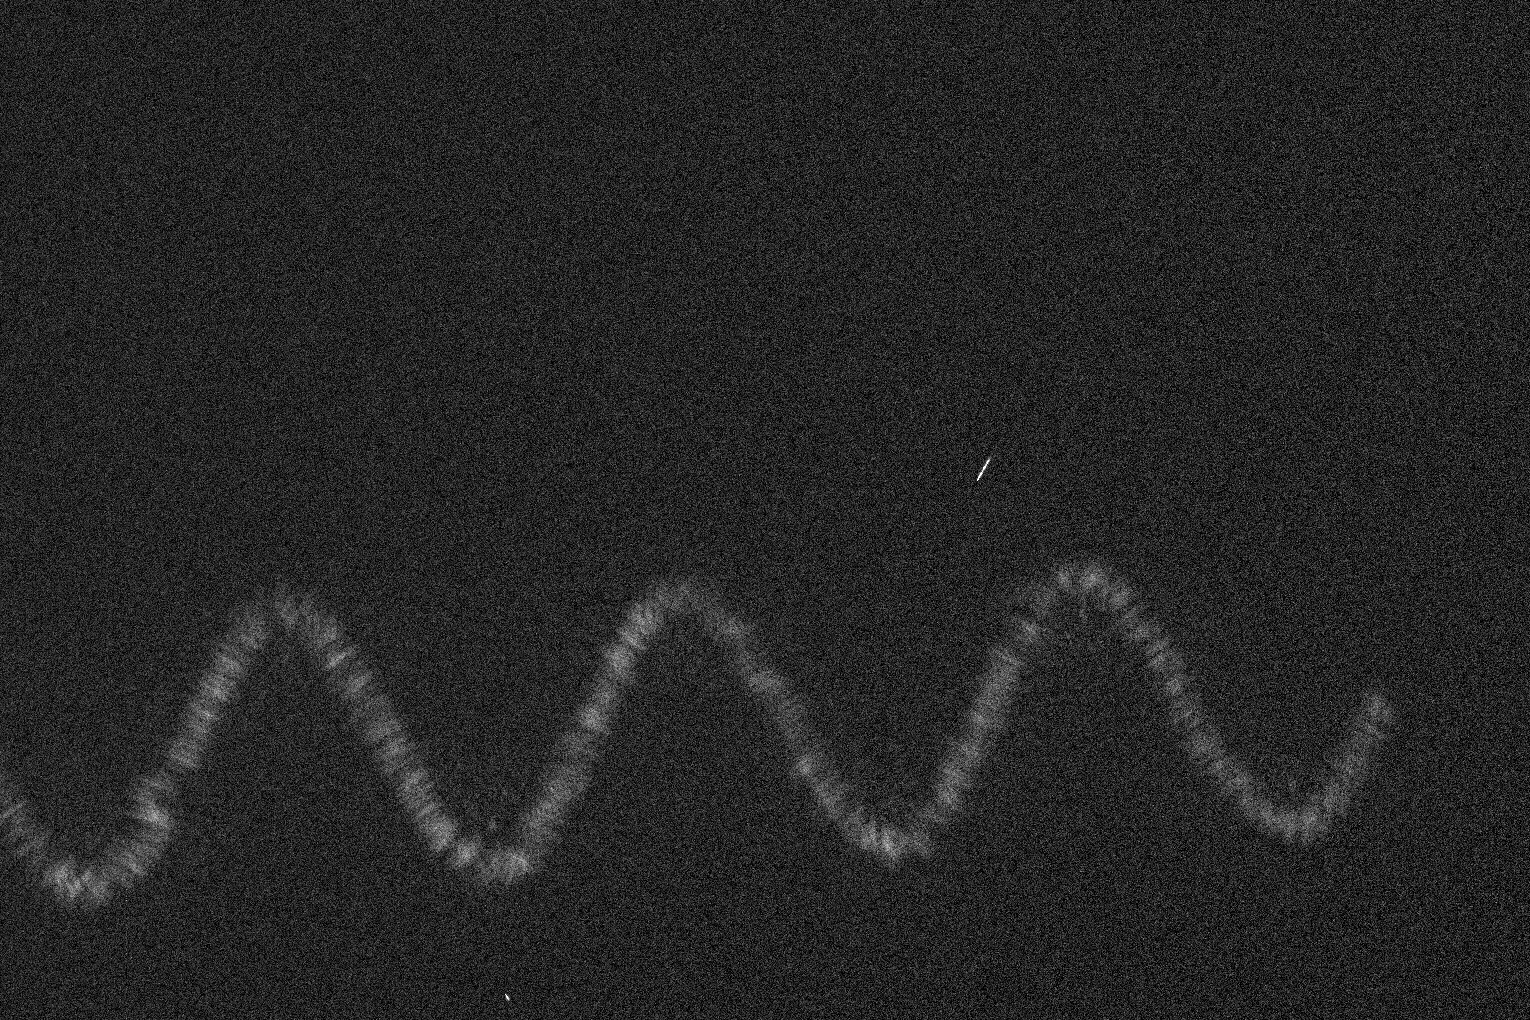
\includegraphics[width=\textwidth]{Daten/sin_1.jpg}
	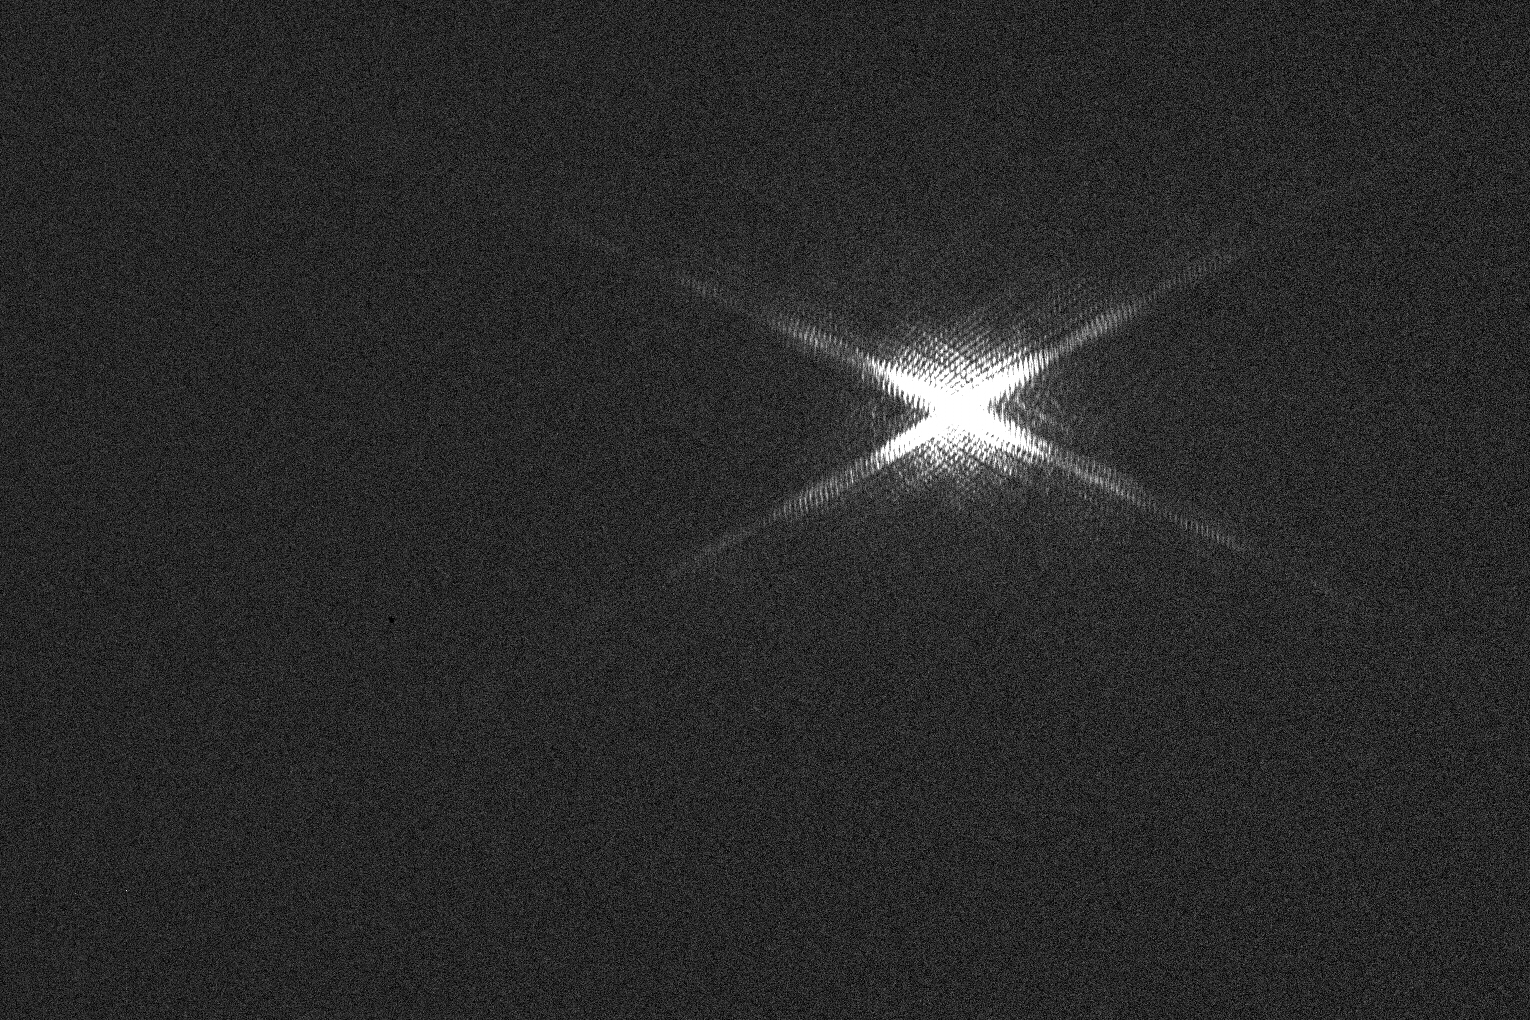
\includegraphics[width=\textwidth]{Daten/sin_2.jpg}
	\caption[Aufnahme Sinus]{Oben echte Abbildung Sinus. Unten Beugungsbild}
\end{figure}
\begin{figure}[h]
	\centering
	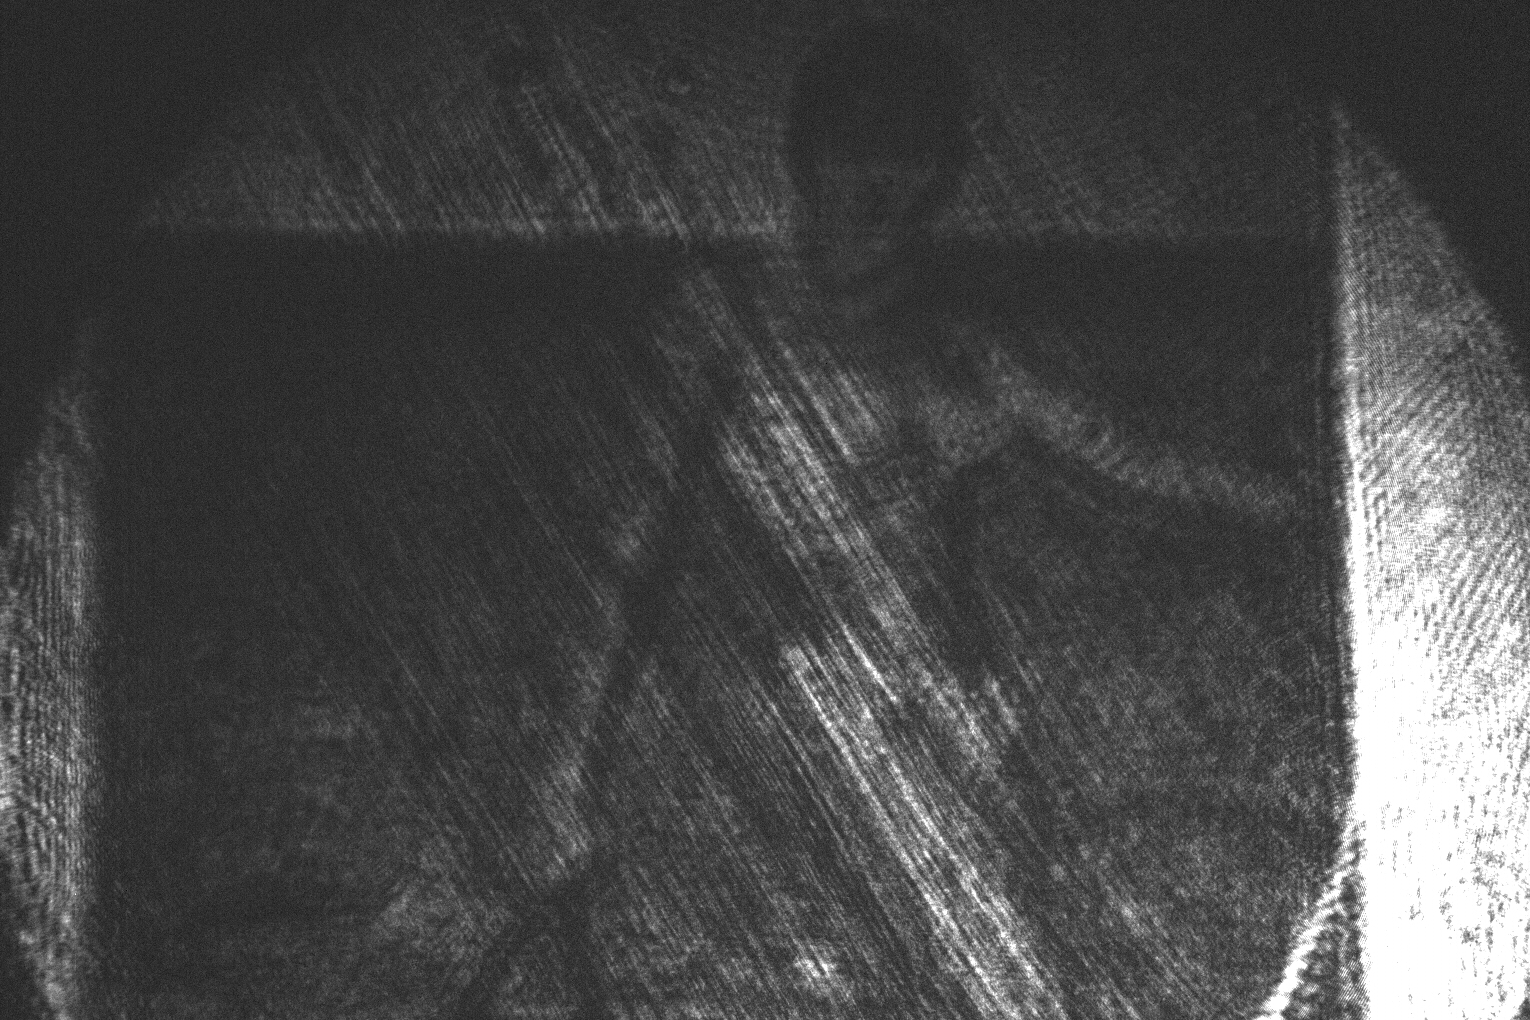
\includegraphics[width=\textwidth]{Daten/frau_1.jpg}
	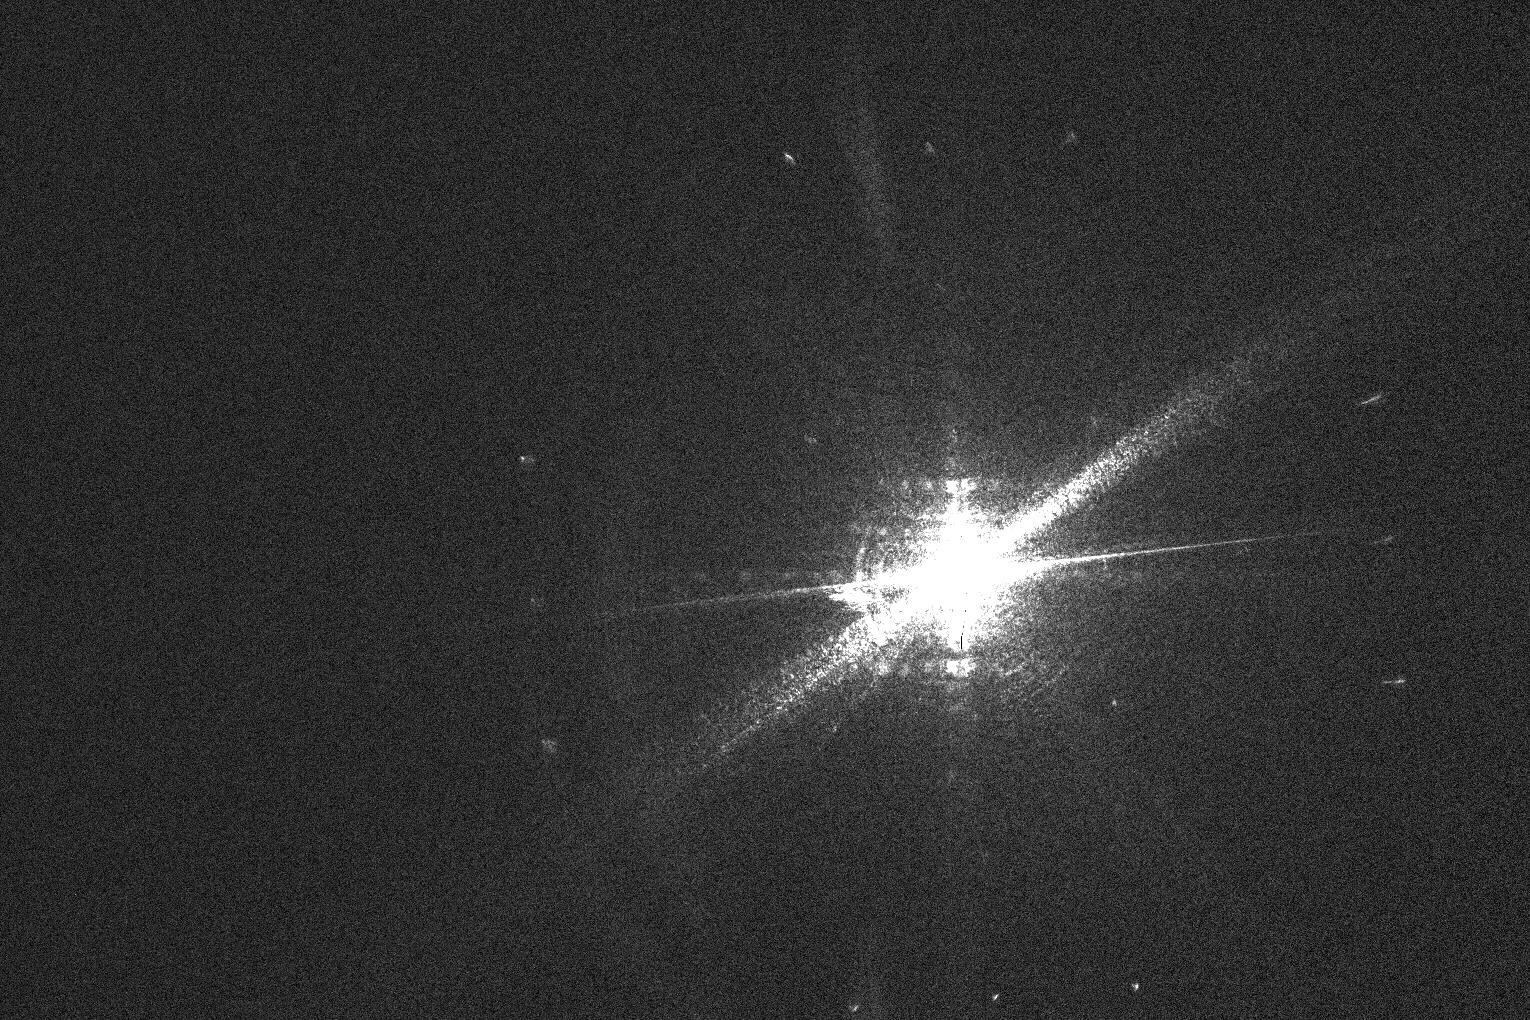
\includegraphics[width=\textwidth]{Daten/frau_2.jpg}
	\caption[Aufnahme Model]{Oben echte Abbildung Bikini Model. Unten Beugungsbild}
\end{figure}
\begin{figure}[h]
	\centering
	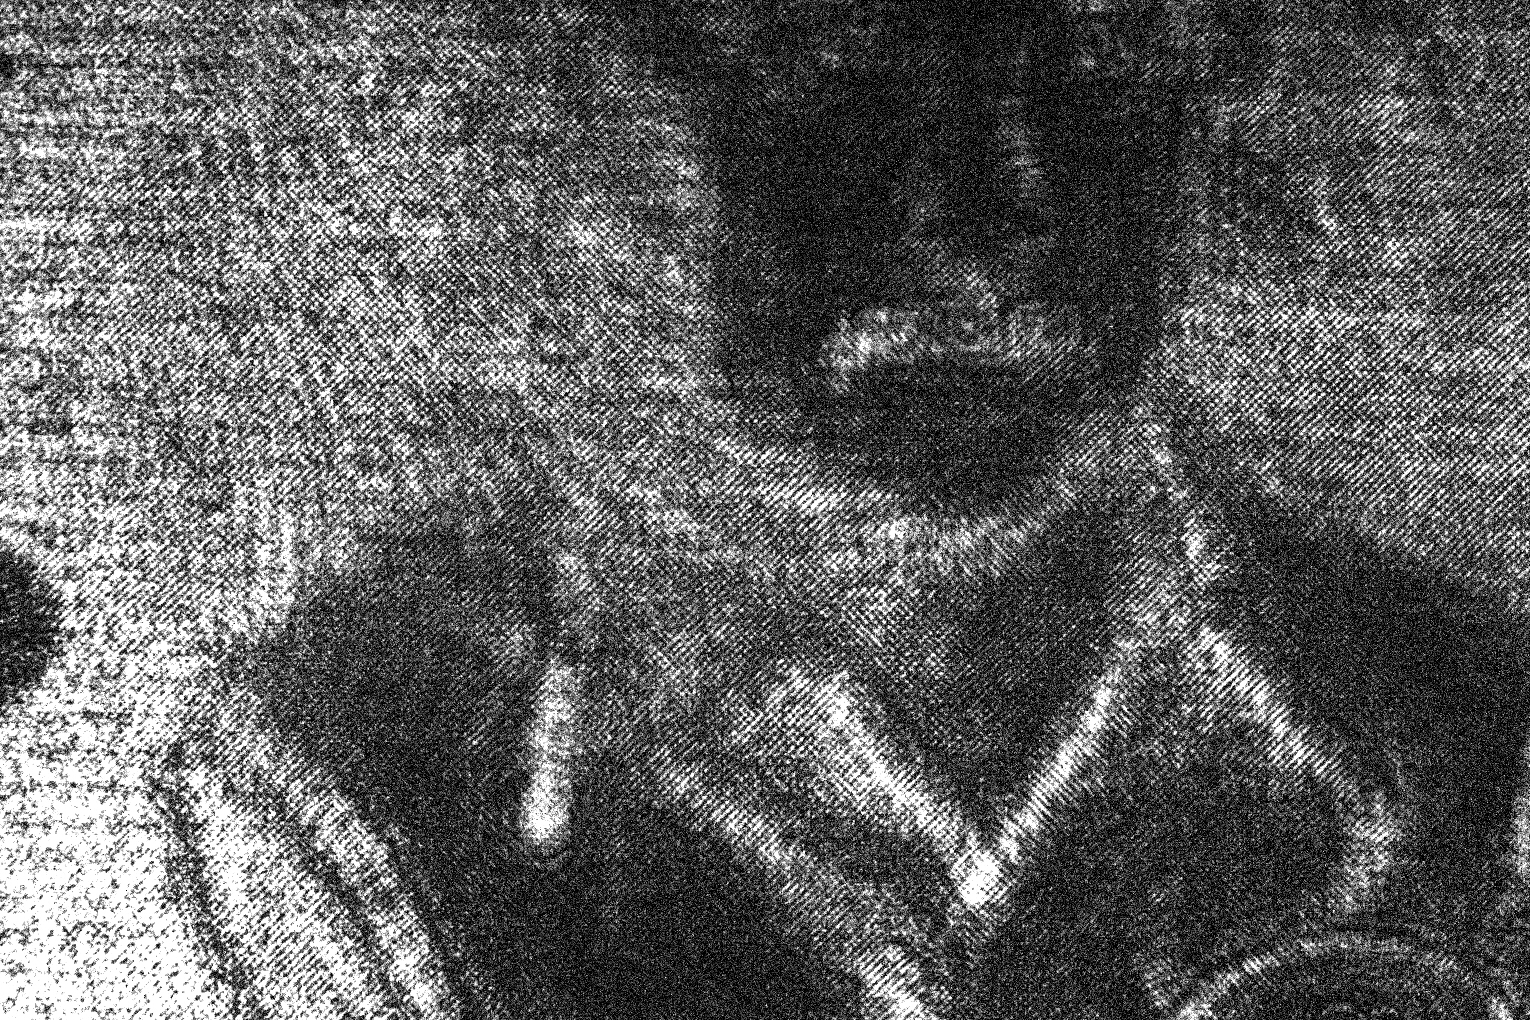
\includegraphics[width=\textwidth]{Daten/einstein_1.jpg}
	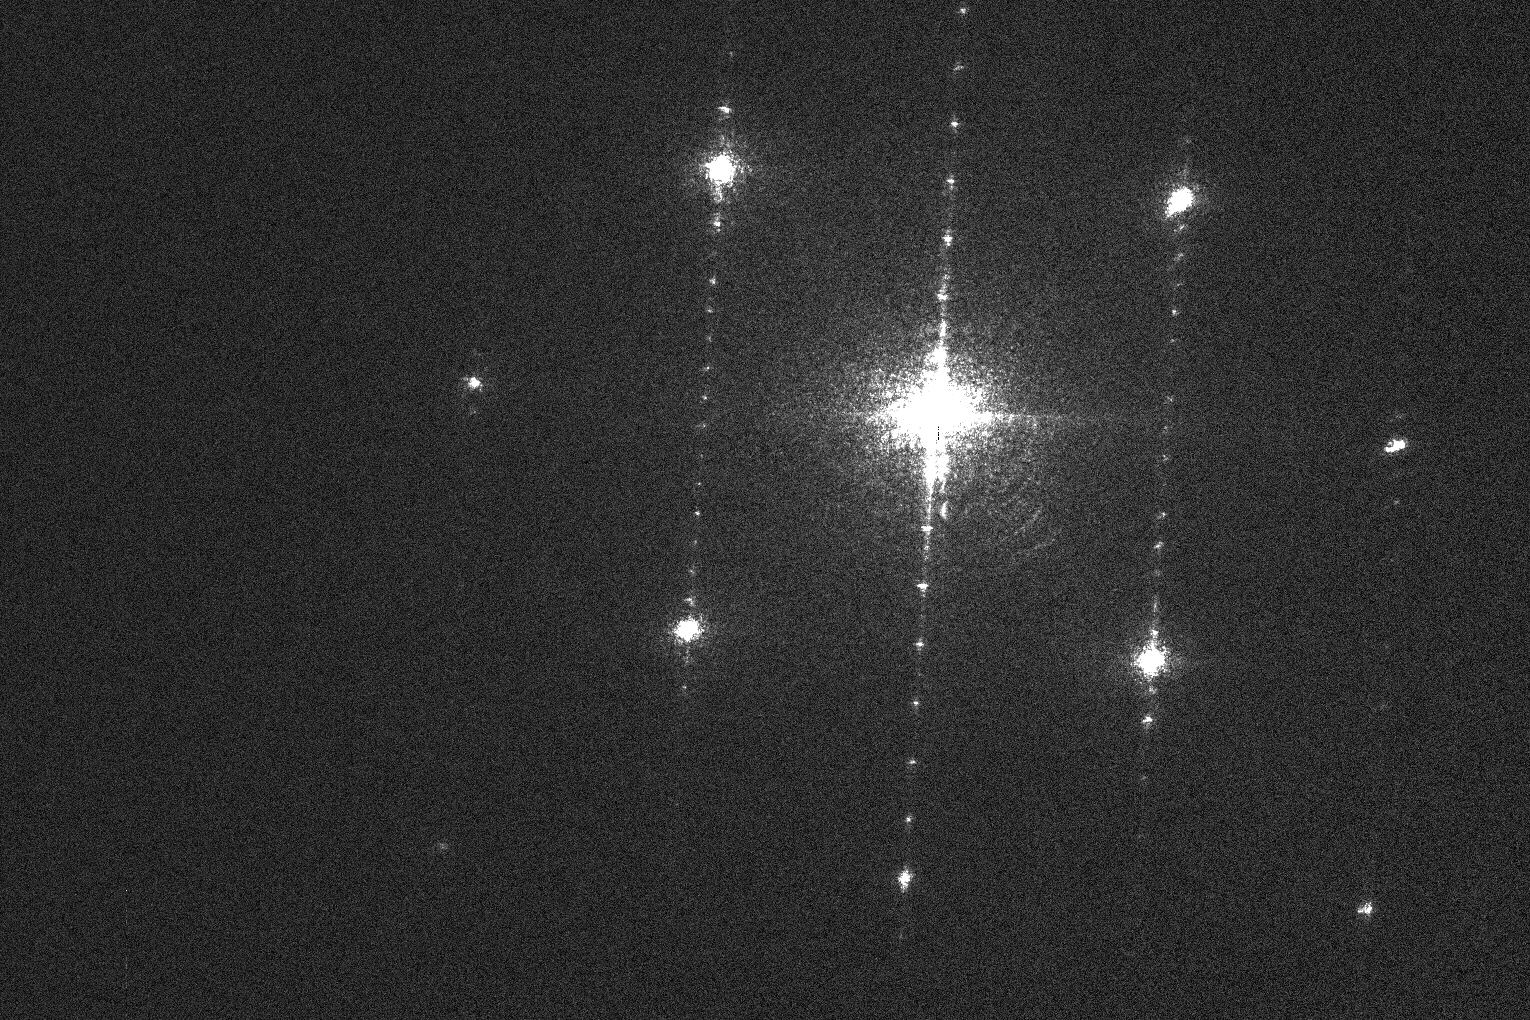
\includegraphics[width=\textwidth]{Daten/einstein_2.jpg}
	\caption[Aufnahme Einstein]{Oben echte Abbildung Einstein. Unten Beugungsbild}
\end{figure}
